\documentclass[11pt,a4paper]{article}

% =========================================================================
% PAKET-PAKET UTAMA
% =========================================================================
\usepackage[utf8]{inputenc}
\usepackage[T1]{fontenc}
\usepackage{lmodern}
\usepackage[indonesian]{babel}
\usepackage{amsmath,amssymb,amsfonts,amsthm}
\usepackage{bm}              % Notasi tebal untuk vektor & matriks
\usepackage{geometry}
\geometry{top=2.5cm, bottom=2.5cm, left=2.5cm, right=2.5cm}
\usepackage{graphicx}
\usepackage{booktabs}        % Tabel profesional
\usepackage{tabularx}
\usepackage{microtype}
\usepackage{tikz}            % Diagram skematis
\usetikzlibrary{matrix,decorations.pathreplacing,calc,positioning}
\usepackage{xcolor}
\usepackage{mdframed}        % Kotak highlight untuk pengerjaan soal
\usepackage{caption}
\usepackage{subcaption}
\usepackage{hyperref}
\hypersetup{
    colorlinks=true,
    linkcolor=blue!70!black,
    citecolor=blue!70!black,
    urlcolor=blue!70!black,
    pdfencoding=auto,
    psdextra
}
\pdfstringdefDisableCommands{%
  \def\boldsymbol#1{#1}%
  \def\bm#1{#1}%
  \def\mathbf#1{#1}%
}

% Makro sitasi sederhana (Rasmussen & Williams, 2006)
\newcommand{\citep}[2][]{(Rasmussen \& Williams, 2006\if\relax\detokenize{#1}\relax\else, #1\fi)}
\newcommand{\citet}[2][]{Rasmussen \& Williams (2006\if\relax\detokenize{#1}\relax\else, #1\fi)}

% Pengaturan penomoran dan teorema
\newtheorem{definisi}{Definisi}[section]
\newtheorem{teorema}{Teorema}[section]
\newtheorem{catatan}{Catatan}[section]

% Path direktori gambar
\graphicspath{{figures/}}

% =========================================================================
% INFORMASI DOKUMEN
% =========================================================================
\title{
    \vspace{-1.2cm}
    \textbf{\Large BIMBINGAN TUGAS AKHIR \#2} \\[0.2em]
}
\begin{document}

\maketitle
\vspace{-0.6cm}

% =========================================================================
% TABEL KONVENSI NOTASI & DIMENSI
% =========================================================================
\begin{table}[h!]
\centering
\small
\caption{Konvensi Notasi dan Dimensi Ruang Aljabar Linier.}
\label{tab:notasi}
\begin{tabularx}{\textwidth}{l c l X}
\toprule
\textbf{Kategori Entitas} & \textbf{Simbol Contoh} & \textbf{Ruang Dimensi} & \textbf{Deskripsi / Peran Matematis} \\
\midrule
Jumlah Training Samples & $N$ & $\mathbb{N}$ & Skalar bulat: Banyaknya observasi dalam training dataset. \\
Jumlah Test Points & $N_*$ & $\mathbb{N}$ & Skalar bulat: Banyaknya lokasi target prediksi/inferensi. \\
Dimensi Input Fitur & $D$ & $\mathbb{N}$ & Skalar bulat: Banyaknya koordinat/fitur pada domain input. \\
\midrule
Titik Input Observasi & $\mathbf{x}_i$ & $\mathbb{R}^{D \times 1}$ & Vektor kolom: Koordinat spasial atau fitur sampel ke-$i$. \\
Matriks Desain Training & $X$ & $\mathbb{R}^{N \times D}$ & Matriks training input bertumpuk, $X = [\mathbf{x}_1, \dots, \mathbf{x}_N]^T$. \\
Matriks Desain Test & $X_*$ & $\mathbb{R}^{N_* \times D}$ & Matriks input test point, $X_* = [\mathbf{x}_{*1}, \dots, \mathbf{x}_{*N_*}]^T$. \\
\midrule
Target Observasi & $y_i$ & $\mathbb{R}$ & Skalar riil: Nilai target dengan galat pada titik $\mathbf{x}_i$. \\
Vektor Target Training & $\mathbf{y}$ & $\mathbb{R}^{N \times 1}$ & Vektor kolom observed training data, $\mathbf{y} = [y_1, \dots, y_N]^T$. \\
Fungsi Laten Training & $\mathbf{f}$ & $\mathbb{R}^{N \times 1}$ & Vektor nilai fungsi murni tanpa galat, $\mathbf{f} = [f(\mathbf{x}_1), \dots, f(\mathbf{x}_N)]^T$. \\
Vektor Galat Observasi & $\boldsymbol{\epsilon}$ & $\mathbb{R}^{N \times 1}$ & Vektor residu galat Gaussian, $\boldsymbol{\epsilon} \sim \mathcal{N}(\mathbf{0}, \sigma_n^2 I_N)$. \\
Fungsi Laten Test & $\mathbf{f}_*$ & $\mathbb{R}^{N_* \times 1}$ & Vektor variabel acak nilai fungsi laten yang diprediksi. \\
\midrule
Kovariansi Antar Training Data & $K(X, X)$ & $\mathbb{R}^{N \times N}$ & Matriks Gram simetris positif semi-definit dari fungsi kernel. \\
Kovariansi Total Training Data & $K_y$ & $\mathbb{R}^{N \times N}$ & Matriks kovariansi dengan galat, $K_y = K(X,X) + \sigma_n^2 I_N$. \\
Kovariansi Training-Test & $K(X, X_*)$ & $\mathbb{R}^{N \times N_*}$ & Matriks kovariansi silang antara training points dan test point. \\
Kovariansi Test-Training & $K(X_*, X)$ & $\mathbb{R}^{N_* \times N}$ & Transpose dari matriks silang, $K(X_*, X) = K(X, X_*)^T$. \\
Kovariansi Antar Test Points & $K(X_*, X_*)$ & $\mathbb{R}^{N_* \times N_*}$ & Matriks kovariansi internal antar sesama test point. \\
\midrule
Faktor Cholesky & $L$ & $\mathbb{R}^{N \times N}$ & Matriks segitiga bawah riil (\textit{lower triangular}), $K_y = L L^T$. \\
Vektor Bobot Prediktif & $\boldsymbol{\alpha}$ & $\mathbb{R}^{N \times 1}$ & Vektor solusi sistem linier, $\boldsymbol{\alpha} = K_y^{-1} \mathbf{y} = L^{-T} L^{-1} \mathbf{y}$. \\
Vektor Mean Prediktif & $\bar{\mathbf{f}}_*$ & $\mathbb{R}^{N_* \times 1}$ & Ekspektasi nilai fungsi posterior pada test point $X_*$. \\
Kovariansi Prediktif & $\operatorname{cov}(\mathbf{f}_*)$ & $\mathbb{R}^{N_* \times N_*}$ & Matriks ketidakpastian posterior pada test point $X_*$. \\
Variansi Individual Test Point & $\mathbb{V}[f_{*j}]$ & $\mathbb{R}^+$ & Skalar variansi marjinal test point ke-$j$, yaitu $[\operatorname{cov}(\mathbf{f}_*)]_{jj}$. \\
\bottomrule
\end{tabularx}
\end{table}

\vspace{0.5cm}

% =========================================================================
% BAGIAN 1: PENDAHULUAN & FILOSOFI BAYESIAN
% =========================================================================
\section{Function-Space View \& Gaussian Process}
\label{sec:filosofi}

\textit{Gaussian Process} (GP) adalah metode non-parametrik yang bekerja langsung pada \textit{function-space} \citep[Bab 2, hlm.~13--15]{rasmussen2006}. Alih-alih mencari nilai parameter atau bobot tertentu, GP langsung memodelkan sebaran probabilitas dari berbagai kemungkinan bentuk fungsi $f(\mathbf{x})$.

\begin{definisi}[\textbf{Gaussian Process} \textnormal{\citep[Definisi 2.1, hlm.~13]{rasmussen2006}}]
Suatu Gaussian Process adalah koleksi variabel acak $\{f(\mathbf{x}) \mid \mathbf{x} \in \mathcal{X}\}$ di mana setiap subset berhingga dari indeks $\{\mathbf{x}_1, \dots, \mathbf{x}_N\}$ menghasilkan distribusi bersama (\textit{joint distribution}) multivariat Gaussian.
\end{definisi}

Secara matematis, karakteristik Gaussian Process ditentukan oleh dua komponen utama, yaitu sebuah fungsi mean $m(\mathbf{x}) \in \mathbb{R}$ dan sebuah fungsi kovariansi/kernel $k(\mathbf{x}, \mathbf{x}') \in \mathbb{R}$ \citep[hlm.~13, Persamaan~(2.13)--(2.14)]{rasmussen2006}:
\begin{align}
m(\mathbf{x}) &= \mathbb{E}[f(\mathbf{x})], \\
k(\mathbf{x}, \mathbf{x}') &= \mathbb{E}\big[ (f(\mathbf{x}) - m(\mathbf{x}))(f(\mathbf{x}') - m(\mathbf{x}')) \big]
\end{align}
sehingga proses stokastik ini dinotasikan sebagai:
\begin{equation}
f(\mathbf{x}) \sim \mathcal{GP}\big(m(\mathbf{x}), k(\mathbf{x}, \mathbf{x}')\big)
\end{equation}

\begin{figure}[h!]
\centering
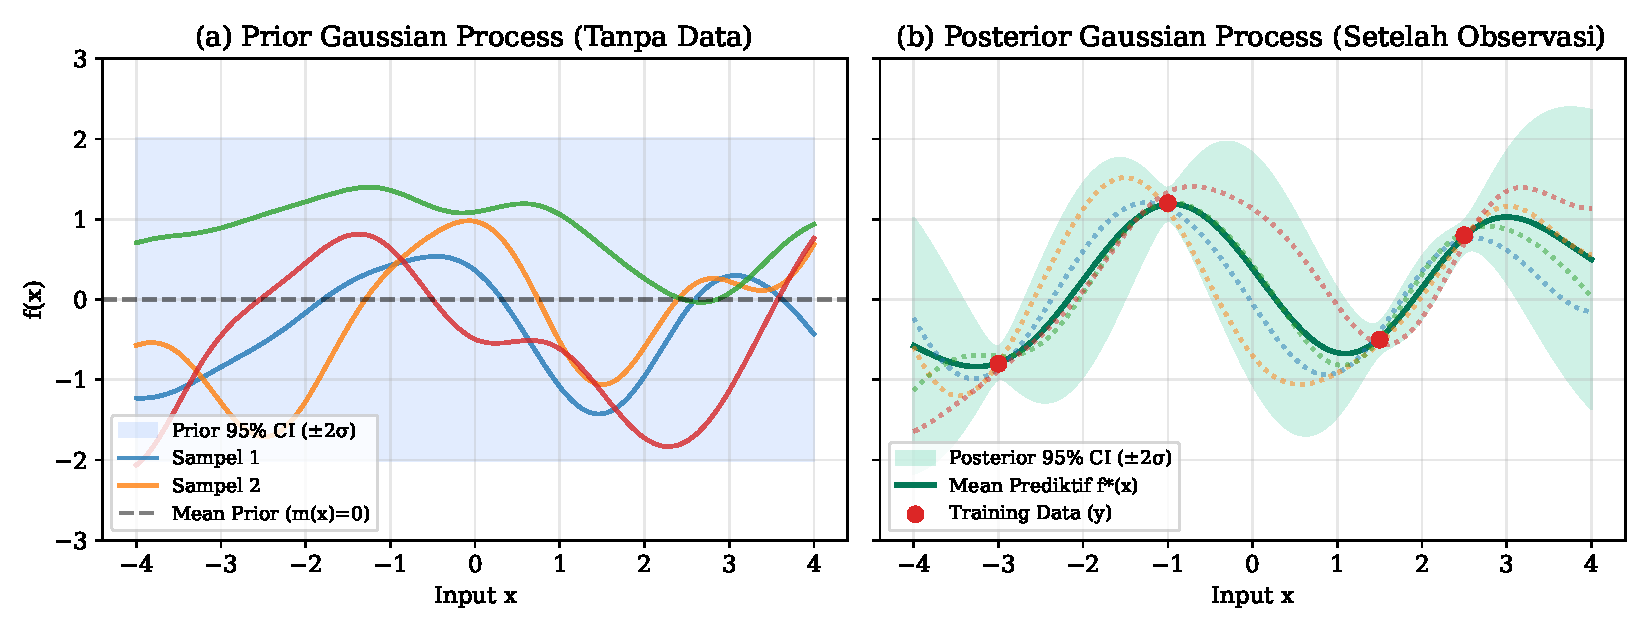
\includegraphics[width=0.95\textwidth]{fig1_prior_posterior.pdf}
\caption{Visualisasi Gaussian Process: (a) Sampel-sampel fungsi prior dari $\mathcal{GP}(0, k(\mathbf{x},\mathbf{x}'))$ dengan pita ketidakpastian konstan $95\%$, dan (b) Sampel-sampel fungsi posterior setelah mengamati empat titik training data, memperlihatkan penyempitan pita ketidakpastian di sekitar titik data.}
\label{fig:prior_posterior}
\end{figure}

% =========================================================================
% BAGIAN 2: KOVARIANSI & FUNGSI KERNEL
% =========================================================================
\section{Covariance Functions (Kernels)}
\label{sec:kernel}

Fungsi kovariansi $k(\mathbf{x}, \mathbf{x}')$ mengukur tingkat kemiripan antara dua titik input: jika nilai input $\mathbf{x}$ dan $\mathbf{x}'$ berdekatan, maka nilai fungsinya $f(\mathbf{x})$ dan $f(\mathbf{x}')$ juga akan bernilai mirip (berkorelasi tinggi).

\subsection{Syarat Kelayakan Kernel (Positive Semi-Definite)}
Agar matriks kovariansi $K \in \mathbb{R}^{N \times N}$ merepresentasikan distribusi Gaussian multivariat yang valid, matriks $K$ wajib bersifat simetris dan positif semi-definit \citep[Definisi 4.1, hlm.~82]{rasmussen2006}. Artinya, untuk setiap himpunan titik $\{ \mathbf{x}_i \}_{i=1}^N$ dan vektor bobot sembarang $\mathbf{v} \in \mathbb{R}^{N \times 1} \setminus \{\mathbf{0}\}$, berlaku:
\begin{equation}
\mathbf{v}^T K \mathbf{v} \ge 0
\end{equation}

\subsection{Kernel Stasioner (\textit{Stationary Kernels})}
Kernel stasioner adalah fungsi kovariansi yang bersifat invarian terhadap translasi input, yaitu nilainya hanya bergantung pada selisih jarak relatif antara dua titik:
\begin{equation}
r = \|\mathbf{x} - \mathbf{x}'\|
\end{equation}

\subsubsection{Kernel Squared Exponential (RBF / Gaussian)}
\begin{equation}
k_{\mathrm{SE}}(\mathbf{x}, \mathbf{x}') = \sigma_f^2 \exp\left( -\frac{\|\mathbf{x} - \mathbf{x}'\|^2}{2 l^2} \right) = \sigma_f^2 \exp\left( -\frac{r^2}{2 l^2} \right)
\end{equation}
Parameter:
\begin{itemize}
    \item $\sigma_f^2$: \textit{signal variance}
    \item $l$: \textit{lengthscale}
\end{itemize}

\subsubsection{Keluarga Kernel Matérn}
\begin{equation}
k_{\mathrm{Mat\acute{e}rn}}(r) = \sigma_f^2 \frac{2^{1-\nu}}{\Gamma(\nu)} \left( \frac{\sqrt{2\nu} r}{l} \right)^\nu K_\nu\left( \frac{\sqrt{2\nu} r}{l} \right)
\end{equation}
Parameter:
\begin{itemize}
    \item $\sigma_f^2$: \textit{signal variance}
    \item $l$: \textit{lengthscale}
    \item $\Gamma(\cdot)$: \textit{gamma function}
    \item $K_\nu(\cdot)$: \textit{modified Bessel function}
\end{itemize}
Bentuk khusus $\nu = 3/2$ dan $\nu = 5/2$:
\begin{itemize}
    \item \textbf{Matérn $\nu = 3/2$}:
    \begin{equation}
    k_{\nu=3/2}(r) = \sigma_f^2 \left( 1 + \frac{\sqrt{3}r}{l} \right) \exp\left( -\frac{\sqrt{3}r}{l} \right)
    \end{equation}
    \item \textbf{Matérn $\nu = 5/2$}:
    \begin{equation}
    k_{\nu=5/2}(r) = \sigma_f^2 \left( 1 + \frac{\sqrt{5}r}{l} + \frac{5r^2}{3l^2} \right) \exp\left( -\frac{\sqrt{5}r}{l} \right)
    \end{equation}
\end{itemize}

\subsection{Kernel Non-Stasioner (\textit{Non-Stationary Kernels})}
Kernel non-stasioner adalah fungsi kovariansi yang nilainya tidak hanya bergantung pada jarak relatif, melainkan bergantung langsung pada posisi absolut dari input $\mathbf{x}$ dan $\mathbf{x}'$ \citep[hlm.~89--90]{rasmussen2006}.

\subsubsection{Kernel Linear}
Kernel linear bersesuaian dengan regresi linear Bayesian \citep[hlm.~89, Persamaan~(4.22)]{rasmussen2006}:
\begin{equation}
k(\mathbf{x}, \mathbf{x}') = \sigma_0^2 + \mathbf{x}^T \mathbf{x}'
\end{equation}
Parameter $\sigma_0^2 \ge 0$ menyatakan variansi dari suku bias/konstanta. Berdasarkan nilai $\sigma_0^2$, kernel linear dibedakan menjadi dua jenis:
\begin{itemize}
    \item \textbf{Homogen}: Jika $\sigma_0^2 = 0$, fungsi kovariansi murni berupa hasil kali titik $k(\mathbf{x}, \mathbf{x}') = \mathbf{x}^T \mathbf{x}'$. Seluruh fungsi sampel linear yang dihasilkan dipaksa melewati titik pusat/origin ($f(\mathbf{0}) = 0$).
    \item \textbf{Inhomogen}: Jika $\sigma_0^2 > 0$, fungsi sampel berupa garis linear sembarang dengan pergeseran vertikal (\textit{intercept}) acak ($f(\mathbf{x}) = \mathbf{w}^T \mathbf{x} + b$).
\end{itemize}
Karena nilainya dipengaruhi langsung oleh magnitudo dan posisi absolut $\mathbf{x}$ serta $\mathbf{x}'$ (bukan selisih jarak $\mathbf{x} - \mathbf{x}'$), kernel linear tergolong non-stasioner.

% =========================================================================
% BAGIAN 3: MODEL REGRESI DENGAN GALAT OBSERVASI
% =========================================================================
\section{Gaussian Process Regression Model}
\label{sec:model_regresi}

Observasi data target sering kali dipengaruhi oleh galat pengukuran \citep[hlm.~16]{rasmussen2006}. Model regresi didefinisikan sebagai:
\begin{equation}
y_i = f(\mathbf{x}_i) + \epsilon_i, \quad i = 1, \dots, N
\end{equation}
di mana residu galat diasumsikan saling bebas dan berdistribusi identik (\textit{i.i.d.}) Gaussian:
\begin{equation}
\epsilon_i \sim \mathcal{N}(0, \sigma_n^2) \implies \boldsymbol{\epsilon} = [\epsilon_1, \dots, \epsilon_N]^T \sim \mathcal{N}(\mathbf{0}_{N \times 1}, \sigma_n^2 I_N)
\end{equation}
di mana $\sigma_n^2 \in \mathbb{R}^+$ adalah variansi galat (skalar) dan $I_N \in \mathbb{R}^{N \times N}$ adalah matriks identitas.

Kovariansi antara dua observasi sembarang $y_p$ dan $y_q$ dapat diturunkan langsung dari sifat ekspektasi linearitas:
\begin{align}
\operatorname{cov}(y_p, y_q) &= \mathbb{E}[(y_p - 0)(y_q - 0)] \nonumber \\
&= \mathbb{E}\big[ (f(\mathbf{x}_p) + \epsilon_p)(f(\mathbf{x}_q) + \epsilon_q) \big] \nonumber \\
&= \mathbb{E}[f(\mathbf{x}_p)f(\mathbf{x}_q)] + \mathbb{E}[f(\mathbf{x}_p)\epsilon_q] + \mathbb{E}[\epsilon_p f(\mathbf{x}_q)] + \mathbb{E}[\epsilon_p \epsilon_q] \nonumber \\
&= k(\mathbf{x}_p, \mathbf{x}_q) + 0 + 0 + \sigma_n^2 \delta_{pq}
\end{align}
di mana $\delta_{pq}$ adalah fungsi delta Kronecker ($\delta_{pq} = 1$ jika $p=q$, dan $0$ jika $p \neq q$).

Dalam notasi matriks penuh, matriks kovariansi observed training data $K_y \in \mathbb{R}^{N \times N}$ dirumuskan sebagai:
\begin{equation}
\label{eq:Ky}
K_y = K(X, X) + \sigma_n^2 I_N \in \mathbb{R}^{N \times N}
\end{equation}
dengan elemen matriks $[K(X, X)]_{ij} = k(\mathbf{x}_i, \mathbf{x}_j)$.

% =========================================================================
% BAGIAN 4: PENURUNAN ANALITIK POSTERIOR
% =========================================================================
\section{Posterior Conditioning \& Inference}
\label{sec:conditioning}

Misalkan diberikan himpunan $N_*$ test input points yang disusun dalam matriks $X_* \in \mathbb{R}^{N_* \times D}$. Tujuan inferensi Bayesian adalah memperoleh distribusi probabilitas bersyarat dari nilai fungsi laten test $\mathbf{f}_* = [f(\mathbf{x}_{*1}), \dots, f(\mathbf{x}_{*N_*})]^T \in \mathbb{R}^{N_* \times 1}$ dengan syarat training data yang diobservasi $(X, \mathbf{y})$, yaitu:
\begin{equation}
p(\mathbf{f}_* \mid X, \mathbf{y}, X_*)
\end{equation}

\subsection{Distribusi Gabungan Prior (Joint Gaussian Prior)}
Berdasarkan definisi dasar Gaussian Process, kumpulan observasi $\mathbf{y} \in \mathbb{R}^{N \times 1}$ dan fungsi laten test $\mathbf{f}_* \in \mathbb{R}^{N_* \times 1}$ secara bersama-sama membentuk distribusi Gaussian multivariat berdimensi $(N + N_*)$ \citep[hlm.~16, Persamaan~(2.21)]{rasmussen2006}:
\begin{equation}
\label{eq:joint_prior}
\begin{bmatrix} \mathbf{y} \\ \mathbf{f}_* \end{bmatrix} \sim \mathcal{N}\left(
\begin{bmatrix} \mathbf{0}_{N \times 1} \\ \mathbf{0}_{N_* \times 1} \end{bmatrix},
\begin{bmatrix}
K_y & K(X, X_*) \\
K(X_*, X) & K(X_*, X_*)
\end{bmatrix}
\right)
\end{equation}
Struktur partisi blok matriks kovariansi pada Persamaan~\eqref{eq:joint_prior} diilustrasikan secara diagramatis pada Gambar~\ref{fig:tikz_joint_matrix}.

\begin{figure}[h!]
\centering
\begin{tikzpicture}[scale=1]
    % Matriks Blok Luar
    \draw[thick, fill=blue!5] (0,0) rectangle (7,7);
    \draw[dashed, line width=1pt, red!70!black] (0,2.5) -- (7,2.5);
    \draw[dashed, line width=1pt, red!70!black] (4.5,0) -- (4.5,7);

    % Label Blok K_y
    \node at (2.25, 4.75) [align=center] {
        \textbf{\large $K_y = K(X,X) + \sigma_n^2 I_N$} \\
        \small Dimensi: $N \times N$ \\
        \footnotesize (Kovariansi Training Data dengan Galat)
    };

    % Label Blok K(X, X_*)
    \node at (5.75, 4.75) [align=center] {
        \textbf{\large $K(X, X_*)$} \\
        \small Dimensi: $N \times N_*$ \\
        \footnotesize (Kovariansi Silang)
    };

    % Label Blok K(X_*, X)
    \node at (2.25, 1.25) [align=center] {
        \textbf{\large $K(X_*, X)$} \\
        \small Dimensi: $N_* \times N$ \\
        \footnotesize ($= K(X, X_*)^T$)
    };

    % Label Blok K(X_*, X_*)
    \node at (5.75, 1.25) [align=center] {
        \textbf{\large $K(X_*, X_*)$} \\
        \small Dimensi: $N_* \times N_*$ \\
        \footnotesize (Prior Titik Test)
    };

    % Anotasi Kurung Kurawal
    \draw [decorate,decoration={brace,amplitude=8pt,mirror,raise=4pt},thick]
    (0,0) -- (4.5,0) node [midway,yshift=-20pt] {\small Training Data $N$};
    \draw [decorate,decoration={brace,amplitude=8pt,mirror,raise=4pt},thick]
    (4.5,0) -- (7,0) node [midway,yshift=-20pt] {\small Test Data $N_*$};

    \draw [decorate,decoration={brace,amplitude=8pt,raise=4pt},thick]
    (0,2.5) -- (0,7) node [midway,xshift=-25pt,rotate=90] {\small Training Data $N$};
    \draw [decorate,decoration={brace,amplitude=8pt,raise=4pt},thick]
    (0,0) -- (0,2.5) node [midway,xshift=-25pt,rotate=90] {\small Test Data $N_*$};
\end{tikzpicture}
\caption{Diagram Partisi Blok Matriks Kovariansi Bersama (\textit{Joint Covariance Matrix}). Matriks berukuran $(N + N_*) \times (N + N_*)$ terbagi menjadi 4 submatriks yang mencerminkan interaksi antara training data dan test data.}
\label{fig:tikz_joint_matrix}
\end{figure}

\subsection{Distribusi Posterior Gaussian Process Regression}
Dengan memanfaatkan teorema pengondisian Gaussian multivariat, distribusi posterior dari fungsi laten test $\mathbf{f}_*$ dengan syarat data observasi $(X, \mathbf{y})$ dirumuskan secara analitik:
\begin{mdframed}[linewidth=1.2pt, linecolor=blue!70!black, backgroundcolor=blue!2]
\textbf{Distribusi Posterior Gaussian Process Regression}:
\begin{equation}
\mathbf{f}_* \mid X, \mathbf{y}, X_* \sim \mathcal{N}\big( \bar{\mathbf{f}}_*, \operatorname{cov}(\mathbf{f}_*) \big)
\end{equation}
\begin{align}
\label{eq:posterior_mean}
\bar{\mathbf{f}}_* &= K(X_*, X) \left[ K(X, X) + \sigma_n^2 I_N \right]^{-1} \mathbf{y} \in \mathbb{R}^{N_* \times 1} \\
\label{eq:posterior_cov}
\operatorname{cov}(\mathbf{f}_*) &= K(X_*, X_*) - K(X_*, X) \left[ K(X, X) + \sigma_n^2 I_N \right]^{-1} K(X, X_*) \in \mathbb{R}^{N_* \times N_*}
\end{align}
\end{mdframed}

Untuk kasus test point tunggal $\mathbf{x}_* \in \mathbb{R}^{D \times 1}$ ($N_* = 1$), notasi disederhanakan dengan $\mathbf{k}_* = K(X, \mathbf{x}_*) \in \mathbb{R}^{N \times 1}$ dan skalar $k_{**} = k(\mathbf{x}_*, \mathbf{x}_*) \in \mathbb{R}$ \citep[hlm.~17, Persamaan~(2.25)--(2.26)]{rasmussen2006}:
\begin{align}
\bar{f}_* &= \mathbf{k}_*^T K_y^{-1} \mathbf{y} \quad \in \mathbb{R} \quad \text{\footnotesize (Dimensi: $(1 \times N) \times (N \times N) \times (N \times 1) = 1 \times 1$)} \\
\mathbb{V}[f_*] &= k_{**} - \mathbf{k}_*^T K_y^{-1} \mathbf{k}_* \quad \in \mathbb{R}^+ \quad \text{\footnotesize (Dimensi: $1 - (1 \times N) \times (N \times N) \times (N \times 1) = 1 \times 1$)}
\end{align}

\end{document}
